\documentclass[12pt]{article}
\usepackage[margin=1in]{geometry}
\usepackage{graphicx}
\usepackage{amsmath}
\usepackage{hyperref}
\usepackage{titlesec}
\usepackage{url}
\titleformat{\section}{\large\bfseries}{\thesection.}{1em}{}
\titleformat{\subsection}{\normalsize\bfseries}{\thesubsection.}{1em}{}

\title{Evaluation of a Logistic Regression Model for Loan Approval Decisions}
\author{}
\date{}

\begin{document}
	
	\begin{titlepage}
	\centering
	\vspace*{2cm}
	
	
\includegraphics[width=0.5\textwidth]{CMU Logo}
	\vspace{1cm}
	
	{\Huge \bfseries Evaluation of a Logistic Regression Model for Loan Approval Decisions \par}
	\vspace{1.5cm}
	
	{\Large Anthony Cade Streich \par}
	\vspace{0.5cm}
	
	CSCI 396: AI Topics \par
	Instructor: Dr. Sherine Antoun \par
	Colorado Mesa University \par
	\vfill
	
	{\large May 2025 \par}
	\end{titlepage}
	
	\section{Introduction}
	This project aims to develop and evaluate an algorithmic decision-making system for loan approval using the German Credit dataset. The main objective is to predict the likelihood of loan default, allowing financial institutions to make informed lending decisions. Logistic Regression was selected because of it's usefulness as a baseline model in machine learning pipelines. Logistic Regression also provides simplicity and effectiveness on smaller datasets [1].  Although real life loan approval models are going to be larger and more complex, this model will provide insight to the challenges one will face when implementing a similar model. In addition to assessing model performance, this project explores fairness, limitations, and ethical concerns to ensure the system aligns with responsible AI practices.
	
	\section{Dataset Overview}
	The dataset is from German Credit Data, a widely recognized benchmarking company in credit risk modeling. It contains 1000 data rows and 20 input columns, including demographic, financial, and employment-related attributes. Although a small data set, the aim of this project is to explore the implications and impacts of a loan approval model, and 1000 data entries will be enough accomplish our goals [2]. The target variable, \texttt{CreditRisk}, is binary: originally coded as 1 (good) and 2 (bad), it was remapped to 0 (good credit risk) and 1 (bad credit risk) for compatibility with scikit-learn conventions.
	
	Categorical features include variables like \texttt{StatusCheckingAcc}, \texttt{CreditHistory}, \texttt{Savings}, and \texttt{ForeignWorker}, while numerical features include \texttt{Duration}, \texttt{CreditAmount}, and \texttt{Age}. The preprocessing pipeline handled categorical features using one-hot encoding, and numerical features were passed through without transformation.
	
	\section{Modeling Approach}
	Although we typically used R-script for exploratory data analysis, this data set has already been preprocessed [1]. Because of this, we can use EDA through python and the scikit-learn library. After this, a Logistic Regression model was implemented, also using the scikit-learn pipeline. The steps included:
	\begin{itemize}
		\item \textbf{Preprocessing:} Categorical columns were one-hot encoded with \texttt{handle\_unknown=\textquotesingle ignore\textquotesingle}.
		\item \textbf{Data splitting:} standard practice splitting with 80\% training and 20\% testing, stratified by target variable.
		\item \textbf{Model training:} Logistic Regression with \texttt{liblinear} solver and \texttt{max\_iter=1000}.
	\end{itemize}
	
	The model outputs probabilities for each class, which are then converted into binary predictions for evaluation.
	
	\section{Model Performance}
	Although this model did not yield the most promising results, these were the highest scores I was able to achieve all semester. The classification report on the test set yielded the following results:
	
	\begin{figure}[h]
		\centering
		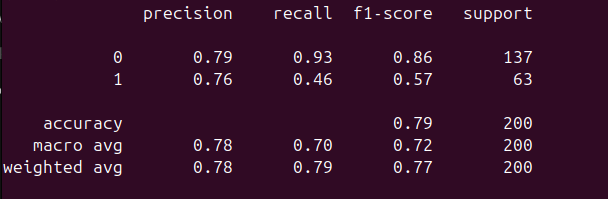
\includegraphics[width=0.8\textwidth]{AccScores.png}
		\label{fig:acc_scores}
	\end{figure}
	
	\begin{itemize}
		\item \textbf{Accuracy:} 79\%
		\item \textbf{Precision (Good Credit Risk):} 79\%
		\item \textbf{Precision (Bad Credit Risk):} 76\%
		\item \textbf{Recall (Good Credit Risk):} 93\%
		\item \textbf{Recall (Bad Credit Risk):} 46\%
		\item \textbf{F1-Score (Good):} 86\%
		\item \textbf{F1-Score (Bad):} 57\%
	\end{itemize}
	
	These results indicate that the model is better at identifying good credit risks than bad ones. The relatively low recall for bad credit risks suggests potential risk in misclassifying risky applicants. This is especially evident after viewing the ROC Curve Graph:
	
	\begin{figure}[h]
		\centering
		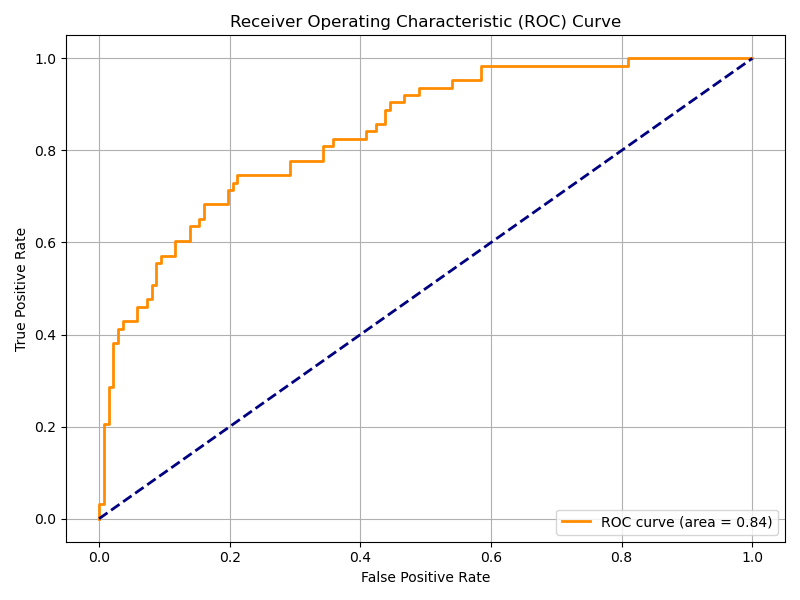
\includegraphics[width=0.5\textwidth]{ROCCurve.png}
	\end{figure}
	
	\section{Feature Importance and Interpretation}
	Logistic regression coefficients were extracted and sorted. Positive coefficients indicate a higher likelihood of loan denial; negative coefficients indicate higher likelihood of approval.
	
	Top positive influencers (more likely to deny):
	\begin{itemize}
		\item \texttt{ForeignWorker = Yes}
		\item \texttt{StatusCheckingAcc = None}
		\item \texttt{CreditHistory = Critical}
		\item \texttt{Job = Unskilled}
		\item \texttt{PersonalStatusSex = Male, Single}
	\end{itemize}
	
	Top negative influencers (more likely to approve):
	\begin{itemize}
		\item \texttt{ExpensiveItem = Owns new car}
		\item \texttt{Savings = Rich}
		\item \texttt{EmploymentSince =\textgreater 7 years}
		\item \texttt{Property = Owns Real Estate}
		\item \texttt{Housing = Own}
		\item \texttt{Telephone = Yes}
	\end{itemize}
	
	\begin{figure}[h]
		\centering
		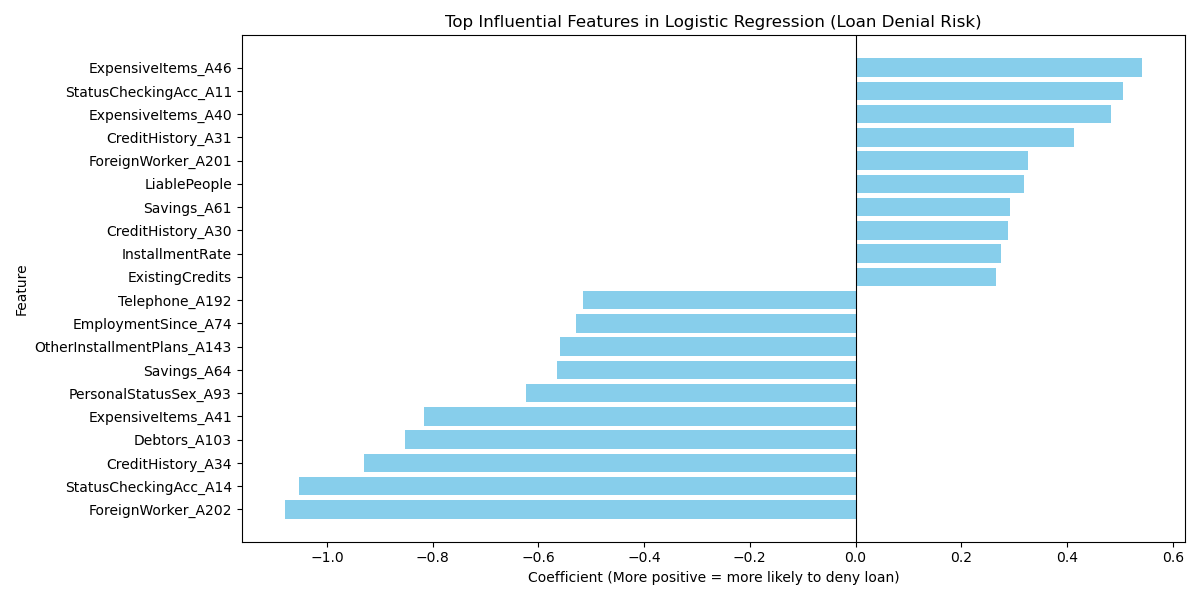
\includegraphics[width=0.8\textwidth]{InfluentialFeatures.png}
		\label{fig:top_features}
	\end{figure}
	
	This visualization reveals an important imbalance: there are more factors that increase the likelihood of loan denial than factors that improve approval odds. While positive indicators (like maintaining a rich savings account or having over seven years of continuous employment) do reduce the risk score, their influence is limited compared to the number and strength of negative risk-related features. This suggests that the model places greater weight on penalizing risk factors rather than rewarding "positive" attributes. As a result, individuals from less privileged backgrounds, who may lack long employment history or significant financial assets, are continuously disadvantaged, reinforcing wealth inequality [3].
	
	\section{Fairness Evaluation}
	Several features in the dataset served as proxies for "combined" attributes:
	\begin{itemize}
		\item \texttt{PersonalStatusSex} encoded gender and marital status.
		\item \texttt{ForeignWorker} encoded nationality.
		\item \texttt{Age} can indirectly disadvantage certain age groups.
	\end{itemize}
	
	The high positive coefficient for \texttt{ForeignWorker = Yes} raises fairness issues, with similar concerns applying to gender-encoded features. Mitigation strategies include removing sensitive features, applying fairness-aware algorithms, or post-processing outputs.
	
	\section{Limitations}
	\begin{itemize}
		\item \textbf{Linearity Assumption:} Logistic Regression assumes linearity. This means that the model doesn't automatically map complex interactions or non-linear effects (like diminishing returns or thresholds).
		\item \textbf{High Dimensionality:} One-hot encoding increases dimensionality, risking memory constraints, but this only becomes an issue with larger data sets.
	\end{itemize}
	
	\section{Ethical and Societal Implications}
	Algorithmic loan approval offers efficiency but also risks:
	\begin{itemize}
		\item \textbf{Discrimination:} Sensitive features may cause disparate treatment.
		\item \textbf{Transparency:} Logistic Regression is explainable, but excessive dummy variables reduce clarity.
		\item \textbf{Accountability:} Models must be audited regularly, preferably by an unbiased third party [4].
	\end{itemize}
	
	\section{Conclusion and Future Directions}
	The model performs moderately well but presents fairness and ethical challenges. While interpretable, it relies on features that may bias results. 
	
	Improvements include:
	\begin{itemize}
		\item Excluding sensitive features.
		\item Applying fairness constraints.
	\end{itemize}
	
	Future research should incorporate fairness metrics and real-world validation to support the responsible deployment of AI models. Without proper safeguards, deploying this model in a real-world setting could reinforce existing societal biases embedded in the training data, ultimately worsening inequality. According to IBM (2023), over 42\% of enterprises have already implemented AI technologies. This trend is concerning, as public awareness of AI’s negative capabilities remains limited.
	

	\section{Discussion Questions}
	
	\subsection*{Model Fairness and Bias}
	\begin{enumerate}
		\item Should models be allowed to use features like nationality, gender, or age—even if they improve accuracy?
		\item How can we ensure fairness if excluding sensitive features reduces model performance?
	\end{enumerate}
	
	\subsection*{Ethical and Societal Implications}
	\begin{enumerate}
		\item Who should be held accountable when an algorithm denies a loan unfairly—data scientists, institutions, or the model itself?
		\item Do the benefits of automated decision-making outweigh the risks in high-stakes applications like lending?
		\item Should applicants be entitled to a full explanation of their denial—even if the model is complex?
	\end{enumerate}
	
	\subsection*{Broader Impact}
	\begin{enumerate}
		\item How might deployment of this model impact financial inclusion for marginalized communities?
		\item If this model were deployed globally, what cultural or regulatory issues would need to be considered?
	\end{enumerate}
	
	\pagebreak
	
	\section{Sources}
	\begin{enumerate}
		\item Dua, D., \& Graff, C. (n.d.). \textit{Statlog (German Credit Data) Data Set}. UCI Machine Learning Repository. \url{https://archive.ics.uci.edu/dataset/144/statlog+german+credit+data}
		\item Feldman, M., Friedler, S. A., Moeller, J., Scheidegger, C., \& Venkatasubramanian, S. (2015, August). \textit{Certifying and removing disparate impact}. In Proceedings of the 21st ACM SIGKDD International Conference on Knowledge Discovery and Data Mining (pp. 259--268).
		
		\item IBM. (n.d.). \textit{AI decision-making: Where do businesses draw the line?} IBM. \url{https://www.ibm.com/think/insights/ai-decision-making-where-do-businesses-draw-the-line}
		
		\item IEEE Standards Association. (n.d.). \textit{IEEE Global Initiative on Ethics of Autonomous and Intelligent Systems}. \url{https://standards.ieee.org/industry-connections/activities/ieee-global-initiative/}
		
	\end{enumerate}
	
\end{document}
